\chapter{Final Remarks}


\section{Conclusions}

In this thesis, we have effectively demonstrated the power of the kernel cross-spectral approach in approximating the cross-spectral distribution based on the extension of Bochner's theorem, which has significant utility as a single-trial FC estimator. Furthermore, we encapsulated this concept within a custom DL layer, facilitating the integration of KCS-FC into end-to-end DL models KCS-FCnet and posterior IRKCS-FCnet. This required minimal preprocessing steps while achieving superior accuracy compared to other end-to-end DL architectures. Beyond this, we developed a data-driven regularization approach to mitigate the number of connectivities over the adjacency matrix. This approach integrated the concept of cross-information potential from the field of information-theoretic learning, utilizing kernel matrices and the $\alpha = 2$ Renyi's entropy. As such, we successfully avoided the need to obtain the data's probability distribution. Moreover, we employed both qualitative and quantitative interpretability strategies to advocate for improved model transparency, aiding the search for a suitable measure of a model's interpretability. This was accomplished by comparing average drop scores, thereby gaining insights into the interpretability of competing models. \cref{fig:final_comparison} presents a comparison between the state-of-the-art end-to-end EEG-based DL architectures (depicted in blue), and the two newly proposed architectures, KCS-FCnet and IRKCS-FCnet (depicted in green). Both of the proposed solutions outperform the existing architectures in terms of accuracy and are ranked second in terms of parameter quantity. This displays the remarkable capacity of KCS-FC to decode EEG signals. The main conclusions of this study can be summarized as follows. 

\begin{figure}[h!]
    \centering
    \resizebox{0.9\linewidth}{!}{% This file was created with tikzplotlib v0.10.1.
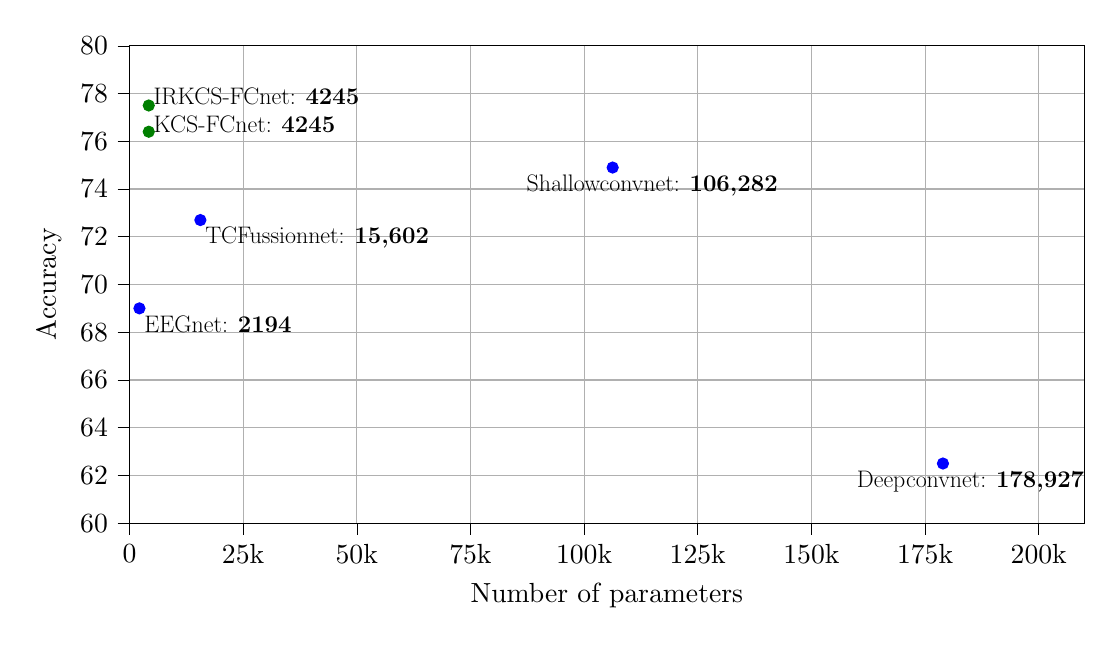
\begin{tikzpicture}

\definecolor{darkgray176}{RGB}{176,176,176}
\definecolor{green01270}{RGB}{0,127,0}

\begin{axis}[
tick align=outside,
tick pos=left,
x grid style={darkgray176},
xlabel={Number of parameters},
ylabel={Accuracy},
xmin=0, xmax=210000,
xtick style={color=black},
xtick={0,25000,50000,75000,100000,125000,150000,175000,200000},
xticklabels={0,25k,50k,75k,100k,125k,150k,175k,200k},
y grid style={darkgray176},
ymin=60, ymax=80,
ytick = {60,62,64,66,68,70,72,74,76,78,80},
ytick style={color=black},
grid=both,
%ymajorgrids=true,
% only scale the axis, not the axis including the ticks and labels
scale only axis=true,
scaled x ticks = false,
% set `width' and `height' to the desired values
width=\textwidth,
height=0.5\textwidth,
]
%\draw[step=5mm,black!15!white, very thin] (0,60) grid (200000,80);
\addplot [draw=blue, draw=none, fill=blue, mark=*]
table{%
x  y
2194 69
};
\addplot [draw=green01270, draw=none, fill=green01270, mark=*]
table{%
x  y
4245 76.4
};
\addplot [draw=green01270, draw=none, fill=green01270, mark=*]
table{%
x  y
4245 77.5
};
\addplot [draw=blue, draw=none, fill=blue, mark=*]
table{%
x  y
178927 62.5
};
\addplot [draw=blue, draw=none, fill=blue, mark=*]
table{%
x  y
106282 74.9
};
\addplot [draw=blue, draw=none, fill=blue, mark=*]
table{%
x  y
15602 72.7
};
\draw (axis cs:2194,68) node[
  scale=0.5,
  anchor=base west,
  text=black,
  rotate=0.0
]{\LARGE{EEGnet:  \textbf{2194}}};
\draw (axis cs:4245,76.37) node[
  scale=0.5,
  anchor=base west,
  text=black,
  rotate=0.0
]{\LARGE{KCS-FCnet:  \textbf{4245}}};

\draw (axis cs:4245,77.53) node[
  scale=0.5,
  anchor=base west,
  text=black,
  rotate=0.0
]{\LARGE{IRKCS-FCnet:  \textbf{4245}}};

\draw (axis cs:158927,61.5) node[
  scale=0.5,
  anchor=base west,
  text=black,
  rotate=0.0
]{\LARGE{Deepconvnet:  \textbf{178,927}}};
\draw (axis cs:86282,73.9) node[
  scale=0.5,
  anchor=base west,
  text=black,
  rotate=0.0
]{\LARGE{Shallowconvnet:  \textbf{106,282}}};
\draw (axis cs:15602,71.7) node[
  scale=0.5,
  anchor=base west,
  text=black,
  rotate=0.0
]{\LARGE{TCFussionnet:  \textbf{15,602}}};
\end{axis}

\end{tikzpicture}
}
    \caption{Comparison of state-of-the-art end-to-end EEG-based DL architectures (in blue) with the proposed KCS-FCnet and IRKCS-FCnet architectures (in green) in terms of accuracy and number of parameters. \label{fig:final_comparison}}
\end{figure}

\begin{itemize}
    \item The validation results obtained from three EEG databases—two with MI and one with ME—demonstrate that the proposed single-trial KCS-FC provides highly competitive classifier performance and is less influenced by handcrafted feature extraction steps, such as the tuning of sliding time window length. Moreover, the benefits of interpreting PLV sets appear limited due to their susceptibility to subject variability, resulting in indistinct topographic channel representations, and PLV provides the poorest classifier performance. Conversely, applying the CCF method results in topoplots showing increased activity over the SMR electrodes, in line with expectations for motor-related tasks. Furthermore, the proposed KCS-FC distinctly highlights two symmetrically located channels over each hemisphere's SMR electrodes, while the accuracy using KCS-FC surpasses other comparable FC estimators. Based on these findings, implementing single-trial KCS-FC for decoding motor skills presents promising potential for MI-BCI systems, enabling high accuracy while maintaining the well-established interpretability of the FC matrices.

    \item KCS-FCnet excels at automatically estimating EEG representations, clearly outperforming other end-to-end architectures. Compared to even more complex methods, KCS-FCnet surpasses them in terms of performance. Although slightly more complex than the EEGnet, it has greater accuracy, especially in contrast to architectures with 25 times more parameters, marking it as a highly efficient model. Further, our analysis of results from three distinct natural groups highlighted that high-performance subjects retain more critical connections than their counterparts. It also addresses the issue of BCI inefficiency by enhancing the accuracy of low-performing individuals and only marginally reducing the performance of one low-performing subject. Our findings underscore the KCS-FCnet architecture as a promising DL strategy for EEG-based MI classification. Given its lightweight setup in terms of parameters, this method is well suited to practical BCI applications, suggesting substantial potential for significant advancements in this field.

    \item The IRKCS-FCnet has proven to be an intrinsic interpretable model, providing valuable insight into spatial connections for MI tasks. More specifically, it highlights the contralateral concept of motor-related neurological states that are deeply rooted within the complex brain network. Furthermore, an additional tool, the average drop score, measures the relevancy of the interpretative results. This aspect can facilitate the identification of transparent models by offering a broader comparative framework that encapsulates performance and interpretive analysis. Importantly, we demonstrated that maximizing the cross-information potential regulates the cross-entropy loss function, mitigating spurious connectivities and reducing the number of true connections that fail to distinguish between MI tasks.
  
\end{itemize}


\section{Future Work}

While our contributions reflect high accuracy and interpretability, additional intricate aspects of the proposed method may warrant further analysis. For instance, the feature extraction process could potentially be refined by utilizing more advanced methods for measuring multivariate similarity, such as centered kernel alignment ~\cite{brockmeier2014neural,alvarez2017kernel}. 

Similarly, extracting more information from the time lag, rather than relying solely on an instantaneous relationship, could help handle volume conductive issues as they primarily apply to instantaneous links. This approach may also serve to draw out more information regarding how past times influence the selected channel ~\cite{uribe2019correntropy,bakhshali2020eeg,de2019data}. The current method's reliance on pairwise relationships might also overlook the influence of a third channel on the interaction between two electrodes, thereby hinting at the potential benefit of implementing more complex solutions, such as multivariate approaches, capable of handling the information carried by other electrodes \cite{vidaurre2023novel}. 

This work sets the stage for more intricate studies in the DL domain, such as cross-subject transfer entropy, where gaining information from different subjects could enhance the decoding of MI tasks embedded in EEG recordings, particularly for low-performing individuals \cite{wei2023sub}. Another promising approach would incorporate Riemannian geometry to encapsulate the internal relationships between different channels in the FC matrix's feature extraction process \cite{carrara2023classification}. Given the recent advancements in the field of graph neural networks, it is conceivable to integrate this concept, given our work's heavy reliance on FC matrices, which naturally generate a dynamic graph. This direction can lead to even more nuanced and sophisticated EEG analysis frameworks \cite{ma2023double}.


\section{Academic Products}

\begin{itemize}
    \item García-Murillo, D.G.; Alvarez-Meza, A.; Castellanos-Dominguez, G. Single-Trial Kernel-Based Functional Connectivity for Enhanced Feature Extraction in Motor-Related Tasks. Sensors 2021, 21, 2750. https://doi.org/10.3390/s21082750 (Q1-A1)
    
    \item García-Murillo, D.G.; Álvarez-Meza, A.M.; Castellanos-Dominguez, C.G. KCS-FCnet: Kernel Cross-Spectral Functional Connectivity Network for EEG-Based Motor Imagery Classification. Diagnostics 2023, 13, 1122. https://doi.org/10.3390/diagnostics13061122 (Q2-A2)

    \item García-Murillo, D.G.; Álvarez-Meza, A.M.; Castellanos-Dominguez, C.G. IRKCS-FCnet: Interpretable Regularized Kernel Cross-Spectral Functional Connectivity Network with Qualitative and Quantitative Post-Hoc and Intrinsic Explainability (Enviado)

    \item Github repository containing all notebooks used in this study  \url{https://github.com/dggarciam/PhD_code_reposotory}

\end{itemize}